\section*{Support Vector Machines}

- Vapnik's invention: A training algorithm for optimal margin classifiers


\subsection*{Linear Classifier}

\begin{wrapfigure}{r}{0.6\columnwidth} 
  \centering
  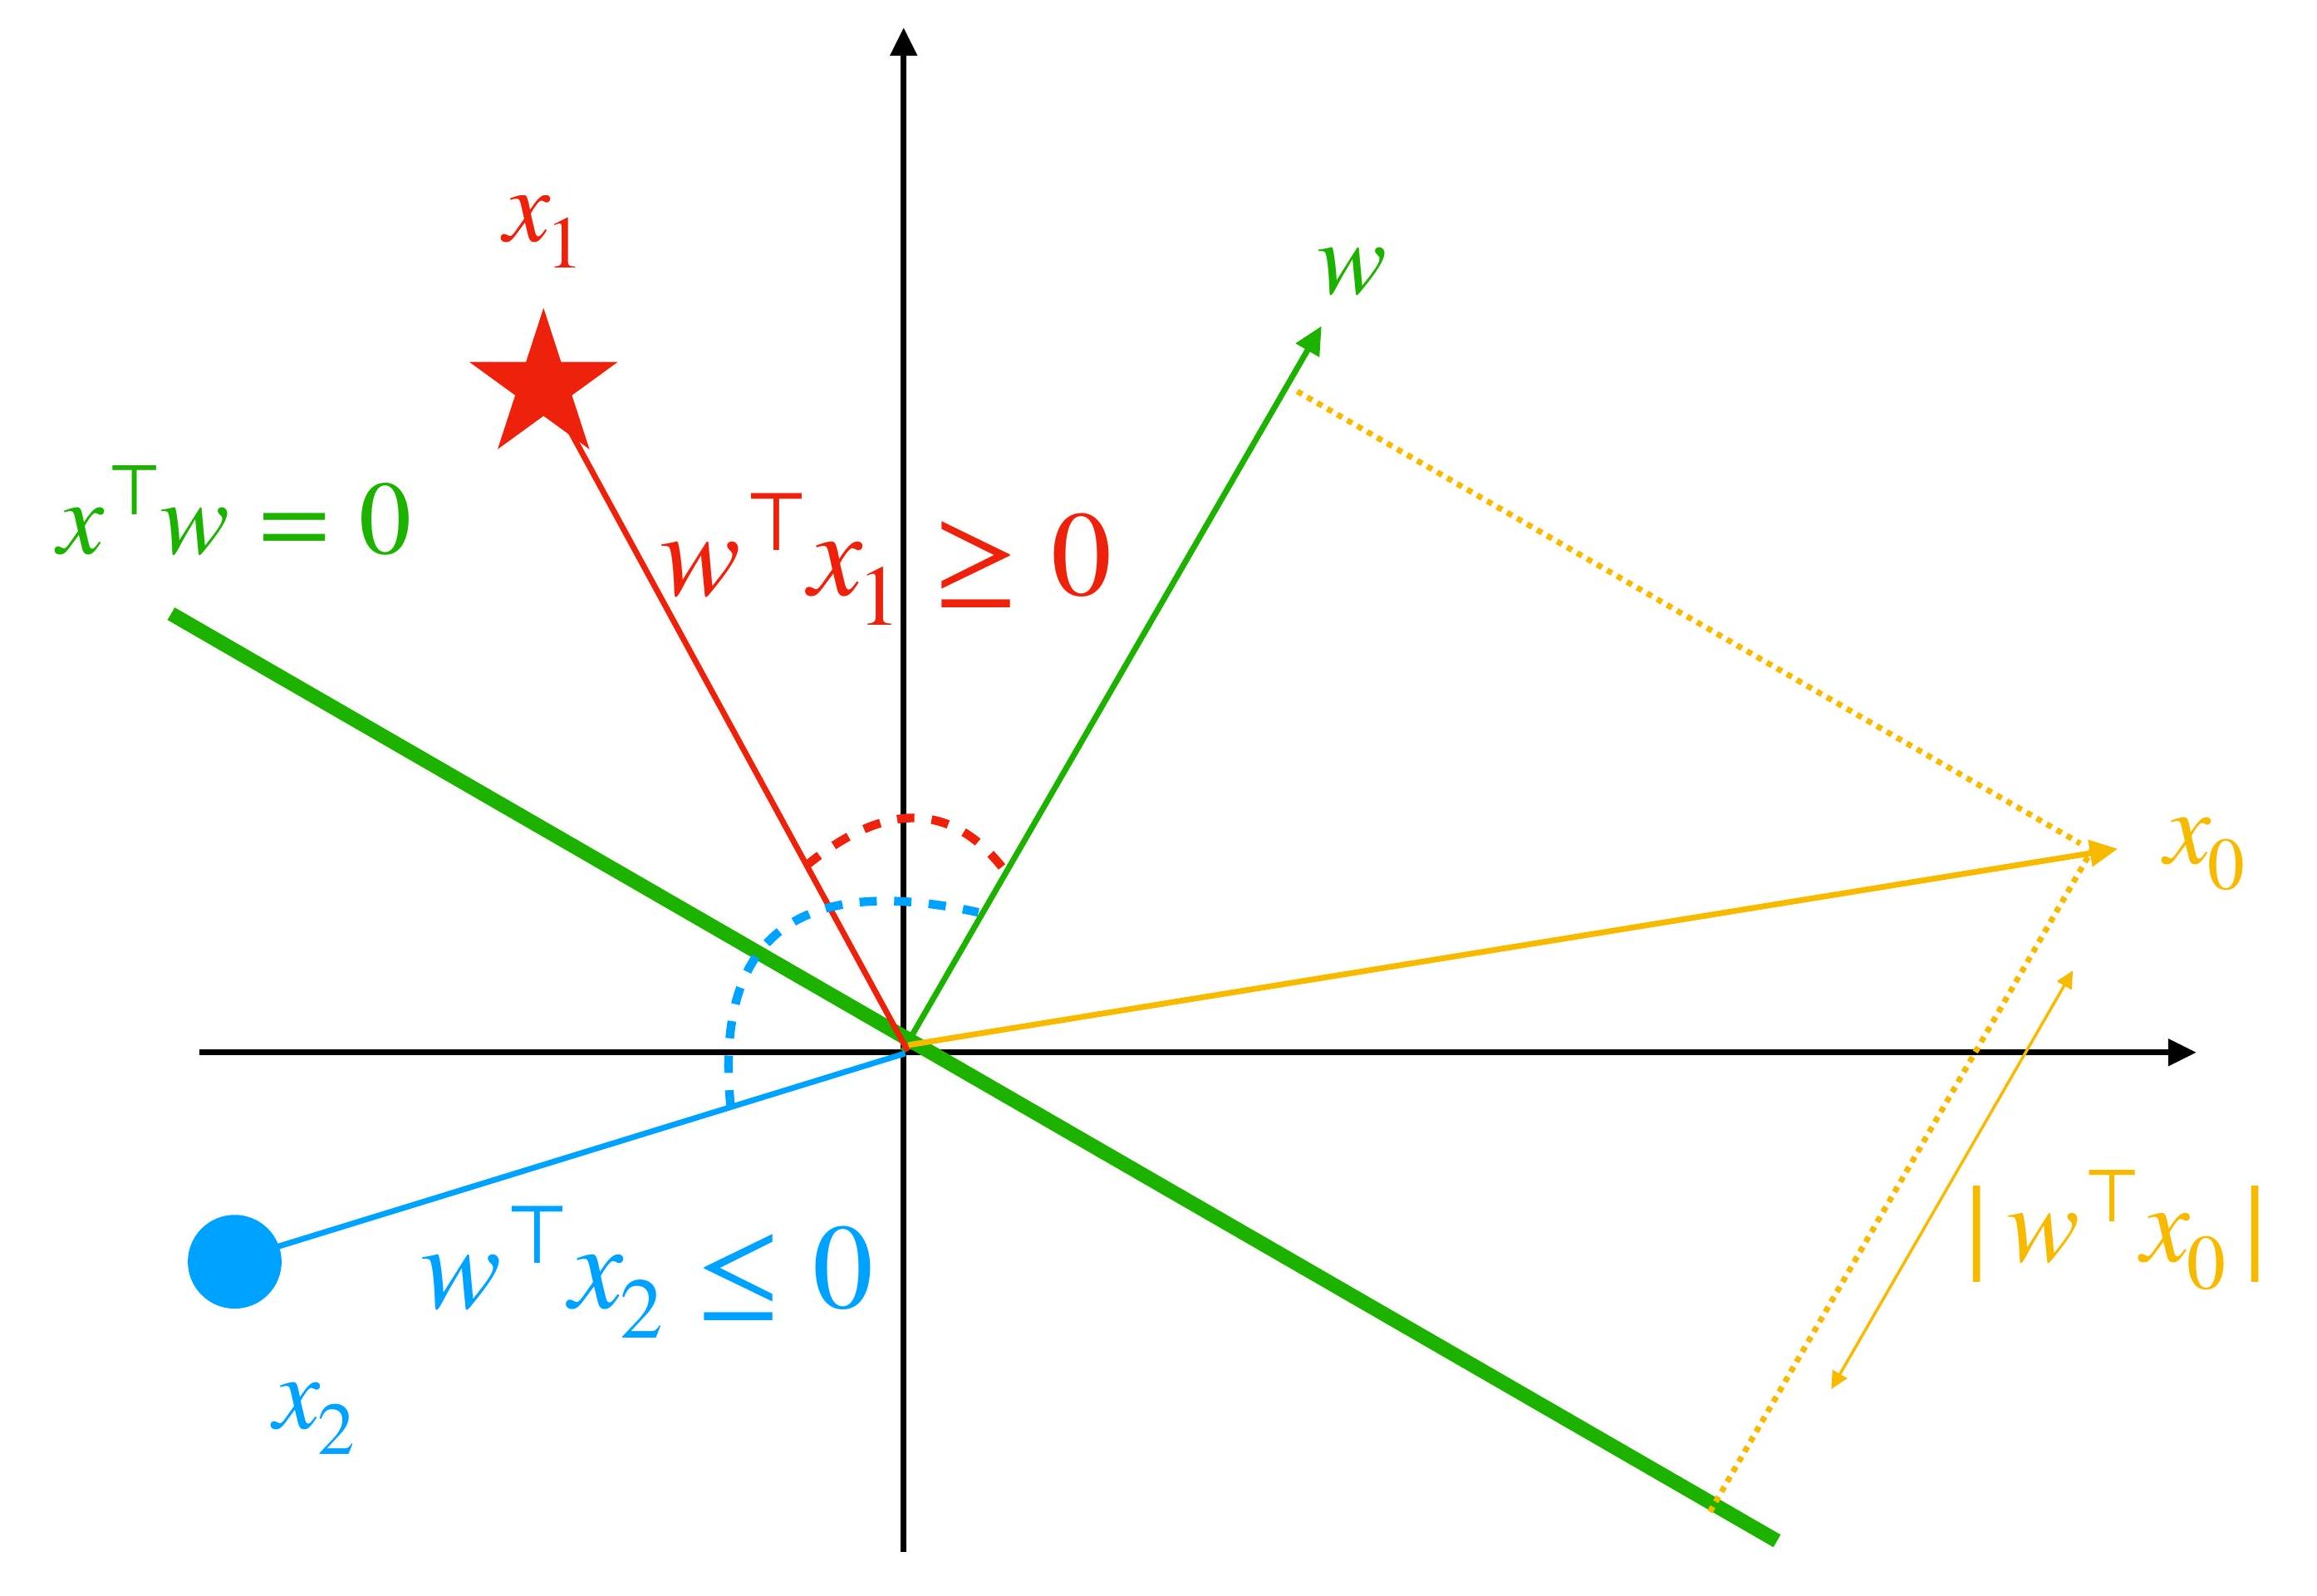
\includegraphics[width=0.6\columnwidth]{figures/hyperplane1.jpg}
\end{wrapfigure}

- Define a hyperplane as $\left\{x: w^{\top} x=0\right\}$ where $\|w\|=1$

- Prediction:

$
f(x)=\operatorname{sign}\left(x^{\top} w\right)
$

- Claim: The distance between a point $x_{0}$ and the hyperplane defined by $w$ is $\left|w^{\top} x_{0}\right|$

- Proof: The distance between $x_{0}$ and the hyperplane is given by $\min _{u: w^{\top} u=0}\left\|x_{0}-u\right\|$

Let $v=x_{0}-w^{\top} x_{0} w$ then by the Pythagorean theorem for any $u$ s.t. $w^{\top} u=0$

% \begin{wrapfigure}{r}{0.6\columnwidth} 
  % \centering
  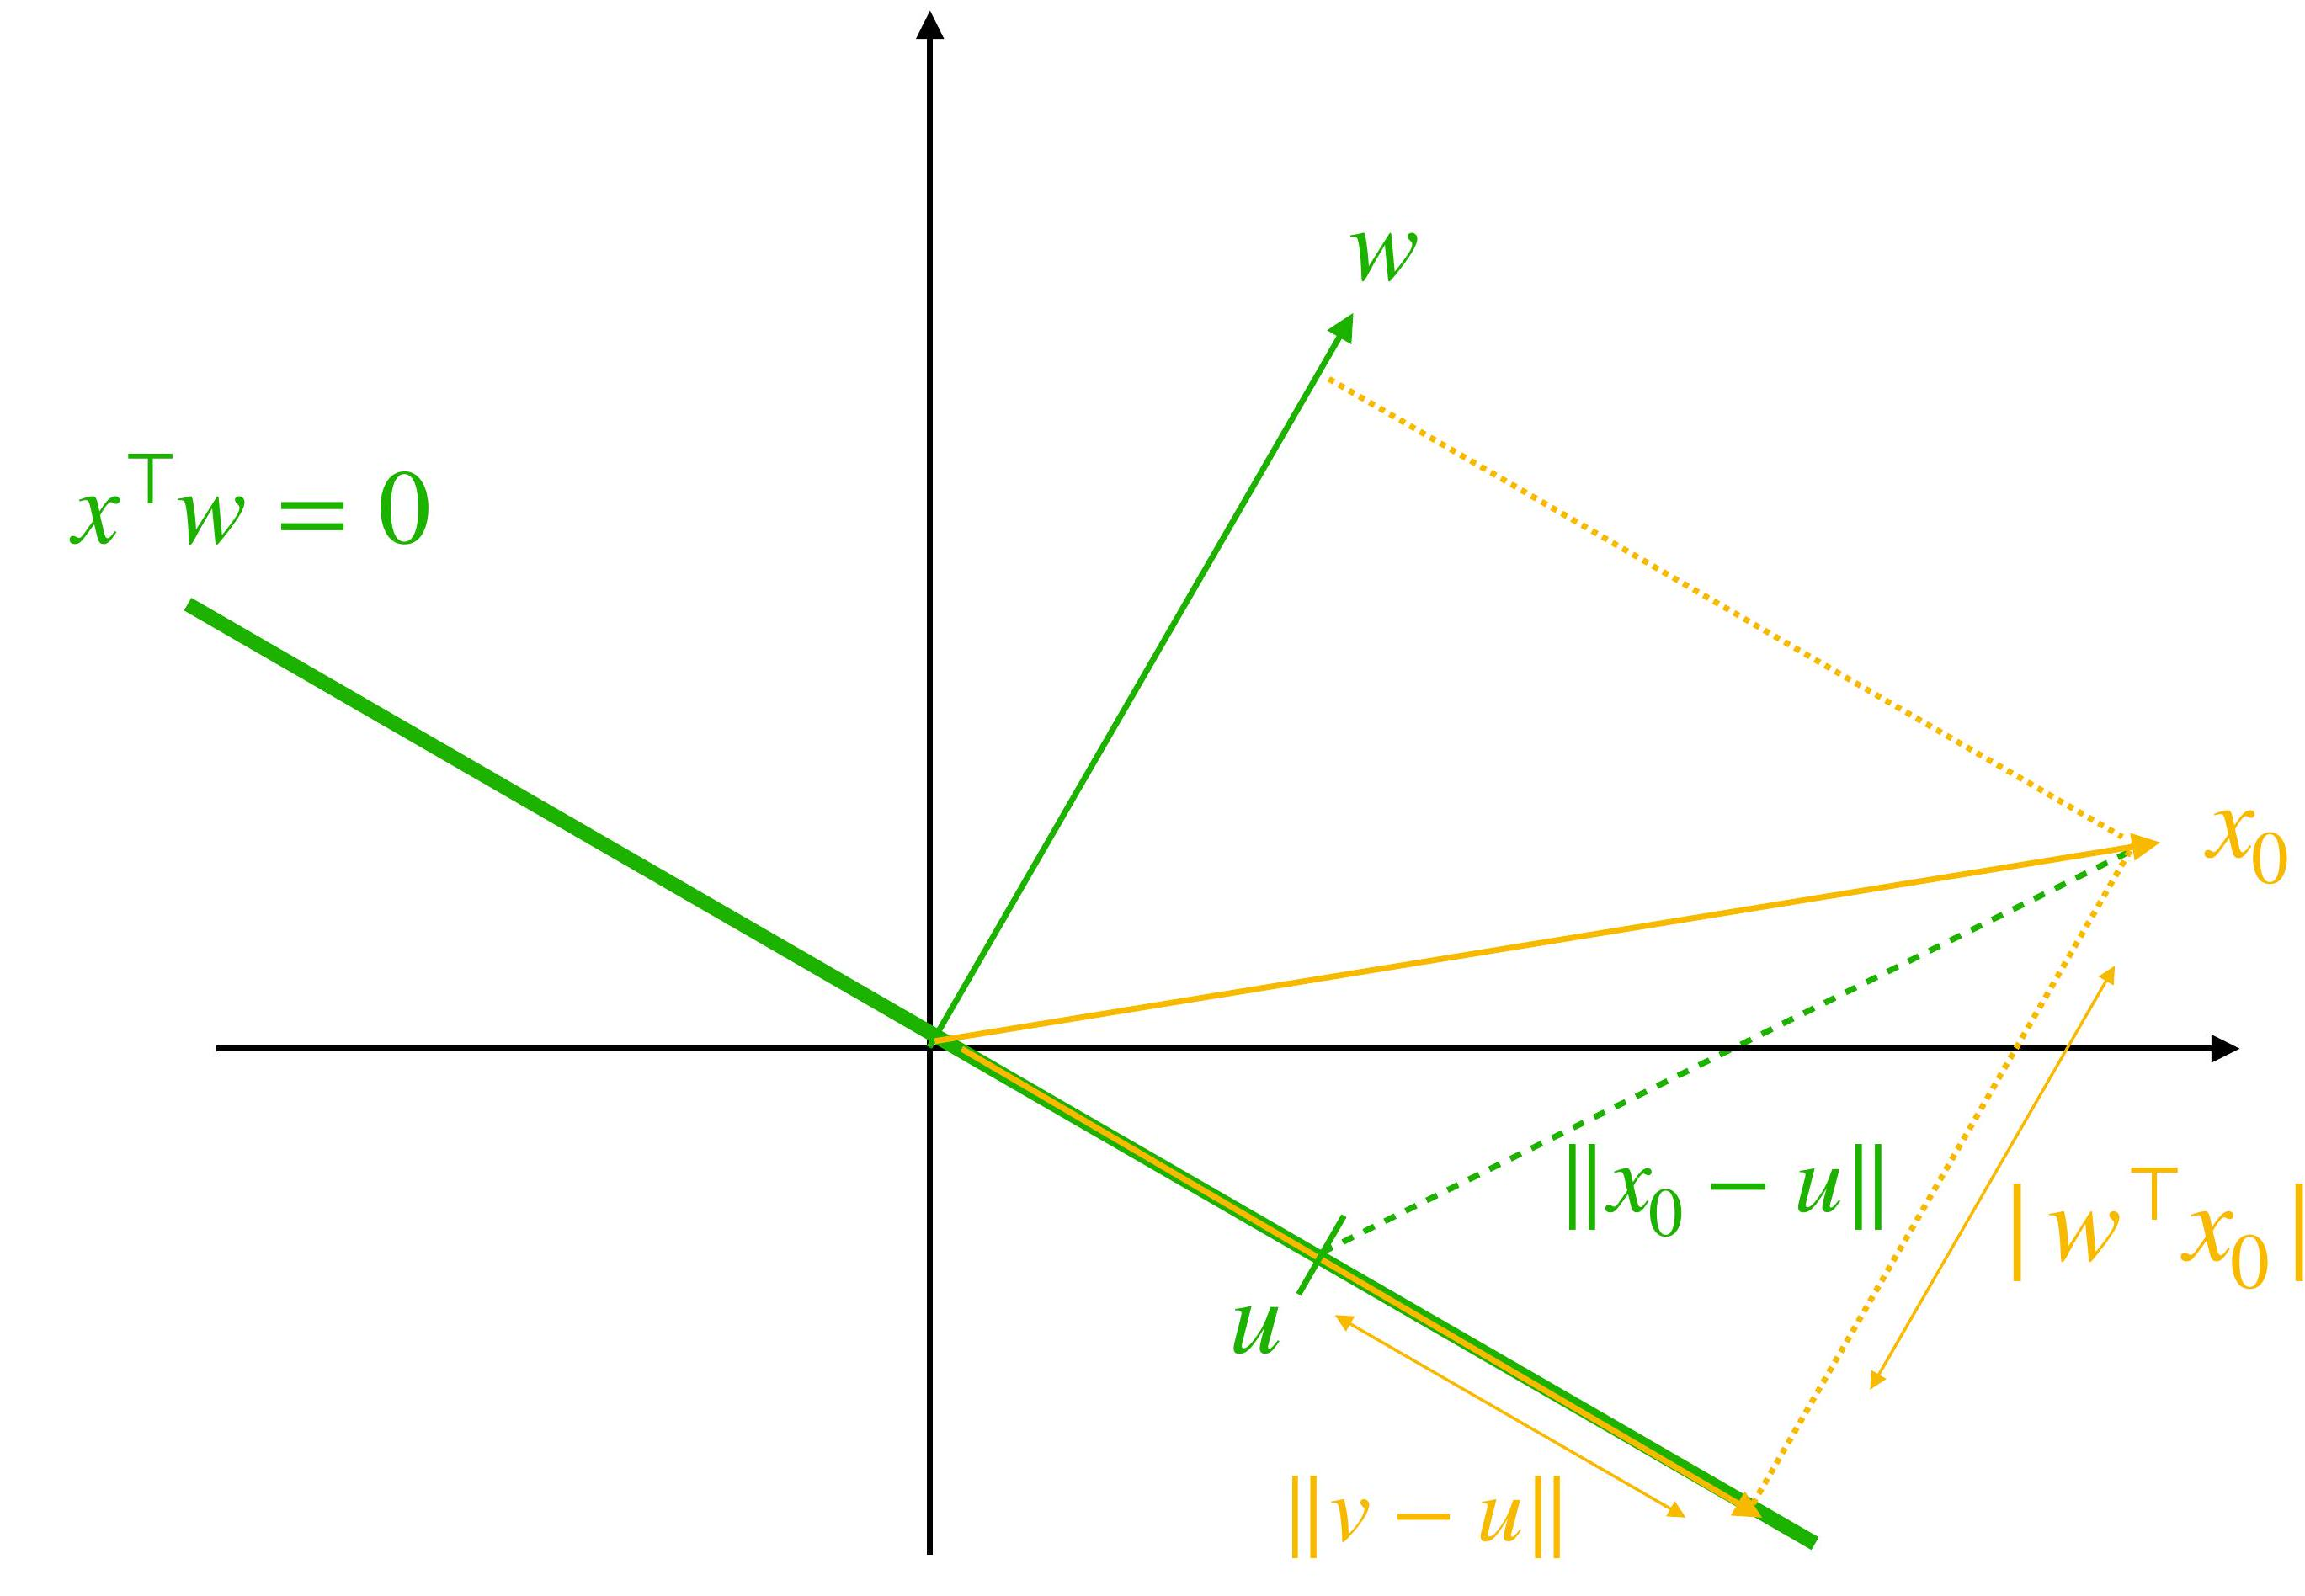
\includegraphics[width=0.9\columnwidth]{figures/hyperplane2.jpg}
% \end{wrapfigure}

$\left\|x_{0}-u\right\|^{2}=\left(w^{\top} x_{0}\right)^{2}+\|v-u\|^{2} \geq\left(w^{\top} x_{0}\right)^{2}$


\subsection*{Hard-SVM rule: max-margin separating hyperplane}

% \begin{wrapfigure}{r}{0.6\columnwidth} 
  % \centering
  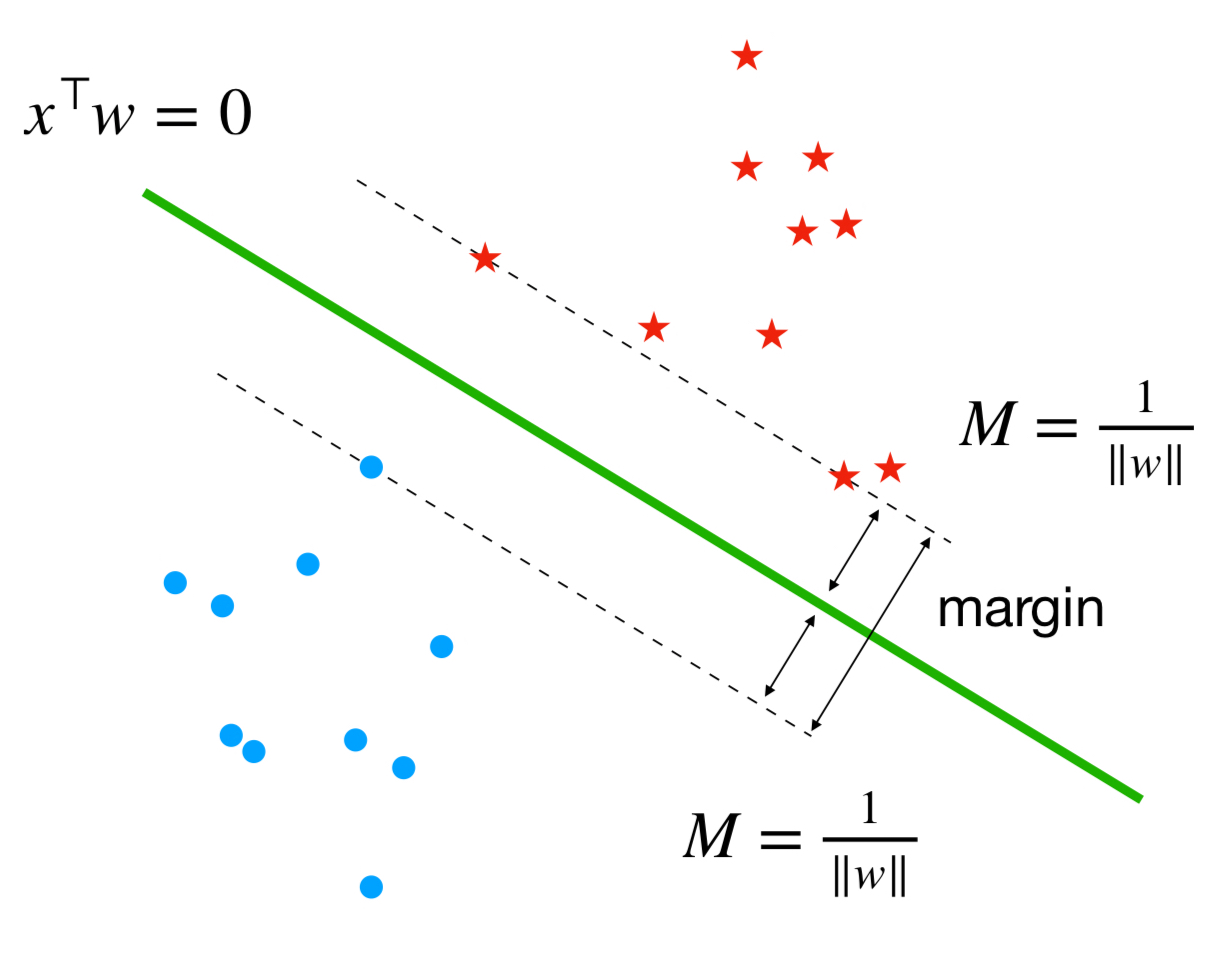
\includegraphics[width=0.8\columnwidth]{figures/hard_svm.jpeg}
% \end{wrapfigure}

- First assume the dataset $\left(x_{n}, y_{n}\right)_{n=1}^{N}$ is linearly separable

- Margin of a hyperplane: $\min _{n \leq N}\left|w^{\top} x_{n}\right|$

- Max-margin separating hyperplane:

$
\max _{w,\|w\|=1} \min _{n \leq N}\left|w^{\top} x_{n}\right| \text { s.t. } \forall n, y_{n} x_{n}^{\top} w \geq 0
$

- Equivalent to: \\$\max _{M \in \mathbb{R}, w,\|w\|=1} M$ s.t. $\forall n, y_{n} x_{n}^{\top} w \geq M$

- Also equivalent to:

$
\min _{w} \frac{1}{2}\|w\|^{2} \text { such that } \forall n, y_{n} x_{n}^{\top} w \geq 1
$

% \subsection*{Proof of the equivalent formulations}
% Claim: The following optimization problems are equivalent
% $\max \min \left|w^{\top} x_{n}\right|$
% $w,\|w\|=1 \quad n \leq N$
% s.t. $\forall n, y_{n} x_{n}^{\top} w \geq 0$
% $\max _{M \in \mathbb{R}, w,\|w\|=1} M$
% s.t. $\forall n, y_{n} x_{n}^{\top} w \geq M$

% Proof: Let $w_{1}$ be a solution of (I) and $M_{1}=\min _{n \leq N}\left|w_{1}^{\top} x_{n}\right|$ and let $w_{2}$ and $M_{2}$ be solutions of (II)

% \begin{itemize}
%   \item $\left(w_{1}, M_{1}\right)$ is admissible for (II) so $M_{1} \leq M_{2}$
%   \item $w_{2}$ is admissible for (I) so $\min _{n \leq N}\left|w_{2}^{\top} x_{n}\right| \leq \min _{n \leq N}\left|w_{1}^{\top} x_{n}\right|$
%   \item $\forall n, y_{n} x_{n}^{\top} w_{2} \geq M_{2}$ implies that $\forall n,\left|x_{n}^{\top} w_{2}\right| \geq M_{2}$ and $\min _{n \leq N}\left|x_{n}^{\top} w_{2}\right| \geq M_{2}$
% \end{itemize}

% Therefore $M_{1}=\min _{n \leq N}\left|w_{1}^{\top} x_{n}\right| \geq \min _{n \leq N}\left|w_{2}^{\top} x_{n}\right| \geq M_{2} \geq M_{1}$

% And the two problems are equivalent

% \subsection*{Proof of the equivalent formulations}
% Claim: The following optimization problems are equivalent

% $$
% \begin{aligned}
% & \max _{M \in \mathbb{R}, w,\|w\|=1} M \\
% & \text { s.t. } \forall n, y_{n} x_{n}^{\top} w \geq M \\
% & \min _{w} \frac{1}{2}\|w\|^{2} \\
% & \text { s.t. } \forall n, y_{n} x_{n}^{\top} w \geq 1
% \end{aligned}
% $$

% Proof:

% $$
% \begin{aligned}
% & \max _{M \in \mathbb{R}, w,\|w\|=1} M \text { such that } \forall n, y_{n} x_{n}^{\top} w \geq M \\
% \Longleftrightarrow & \max _{M \in \mathbb{R}, w} M \text { such that } \forall n, y_{n} x_{n}^{\top} \frac{w}{\|w\|} \geq M
% \end{aligned}
% $$

% The constraints are independent of the scale of $w$. Set $\|w\|=1 / M$ :

% $\Longleftrightarrow \max 1 /\|w\|$ such that $\forall n, y_{n} x_{n}^{\top} w \geq 1$

% $\Longleftrightarrow \min _{w}^{w} \frac{1}{2}\|w\|^{2}$ such that $\forall n, y_{n} x_{n}^{\top} w \geq 1$

\subsection*{Soft SVM}

% \begin{wrapfigure}{r}{0.6\columnwidth} 
  % \centering
  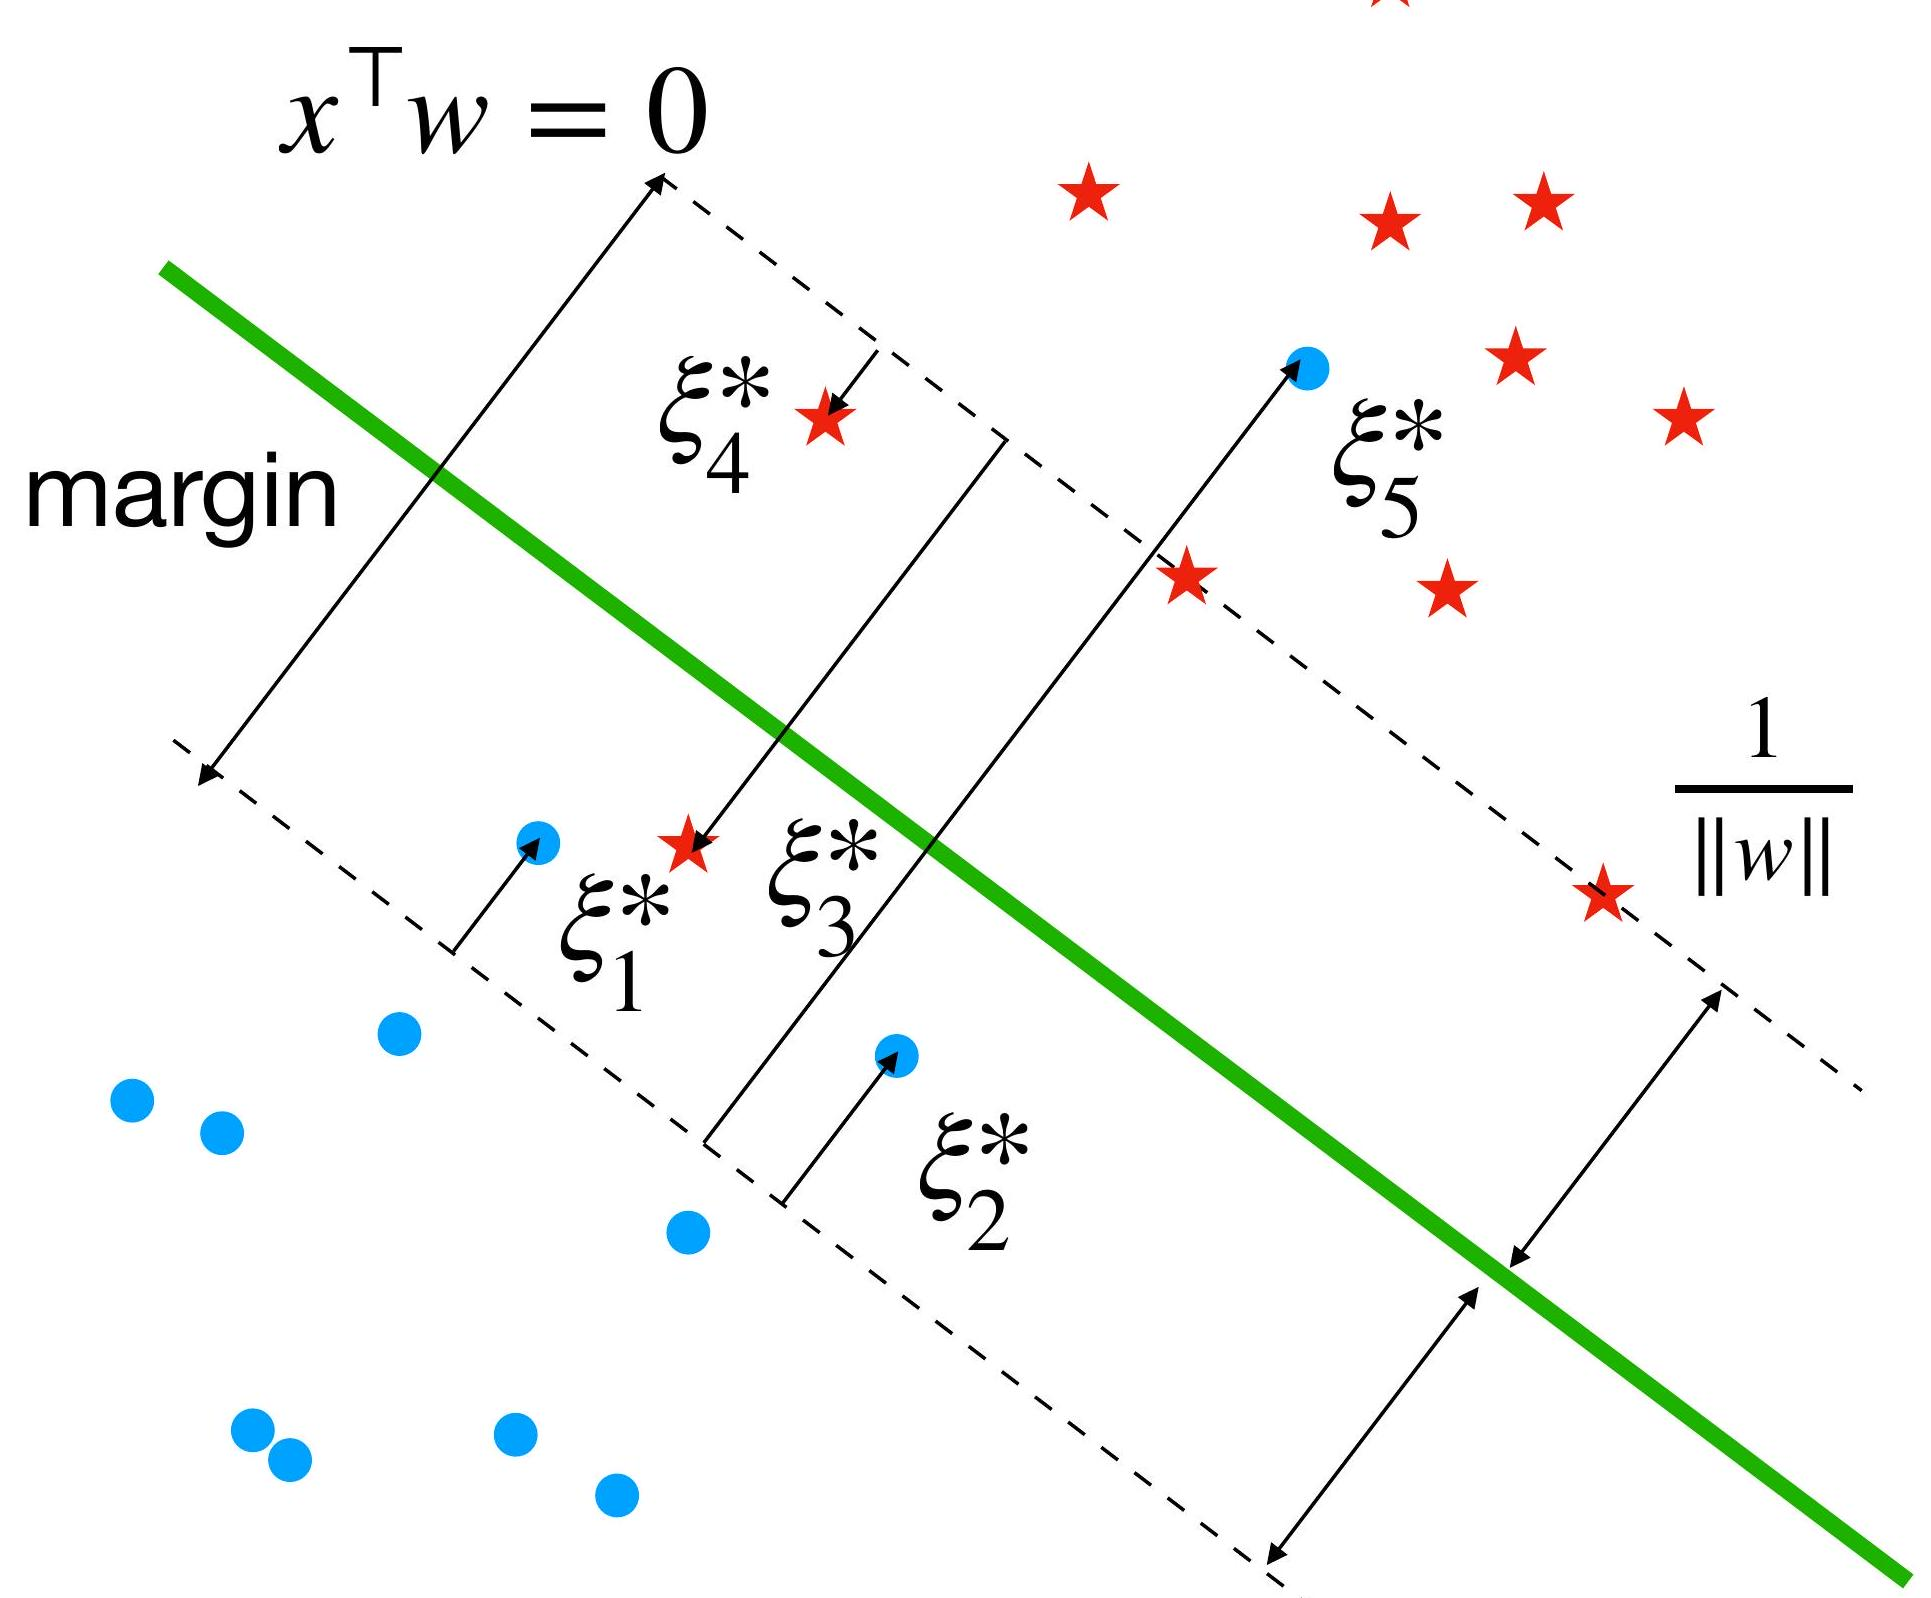
\includegraphics[width=0.7\columnwidth]{figures/soft_svm.jpg}
% \end{wrapfigure}

- A relaxation of the Hard-SVM rule that can be applied even if the training set is not linearly separable

- Idea: Maximize the margin while allowing some constraints to be violated

- Introduce positive slack variables $\xi_{1}, \cdots, \xi_{N}$ and replace the constraints with $y_{n} x_{n}^{\top} w \geq 1-\xi_{n}$ 

- Soft SVM:

$
\begin{aligned}
& \min _{w, \xi} \frac{\lambda}{2}\|w\|^{2}+\frac{1}{N} \sum_{n=1}^{N} \xi_{n} \\
& \text { s.t. } \forall n, y_{n} x_{n}^{\top} w \geq 1-\xi_{n} \text { and } \xi_{n} \geq 0
\end{aligned}
$

- Equivalent to:

$
\min _{w} \frac{\lambda}{2}\|w\|^{2}+\frac{1}{N} \sum_{n=1}^{N}\left[1-y_{n} x_{n}^{\top} w\right]_{+}
$

(A hinge loss)


$
\xi_{i}^{*}=\frac{\xi_{i}}{\|w\|}
$


 
- Proof: Fix $w$ and consider the minimization over $\xi$ :

1) If $y_{n} x_{n}^{\top} w \geq 1$, then $\xi_{n}=0$

2) If $y_{n} x_{n}^{\top} w<1, \xi_{n}=1-y_{n} x_{n}^{\top} w$

Therefore $\xi_{n}=\left[1-y_{n} x_{n}^{\top} w\right]_{+}$


\subsection*{Classification by risk minimization}
- $(X, Y) \sim \mathscr{D}$ with ranges $\mathscr{X}$ and $\mathscr{Y}=\{-1,1\}$

- Goal: Find a classifier $f: \mathscr{X} \rightarrow \mathcal{Y}$ that minimizes the true risk
$
L(f)=\mathbb{E}_{\mathscr{D}}\left(1_{Y \neq f(X)}\right)
$

- How: Through Empirical Risk Minimization (ERM):

$
\min _{w} L_{\text {train }}(w)=\frac{1}{N} \sum_{n=1}^{N} \phi\left(y_{n} w^{\top} x_{n}\right)
$

$\phi$ represents the loss function of the functional margin $y_{n} x_{n}^{\top} w$

$\phi$ also serves as a convex surrogate for the $0-1$ loss

\subsection*{Losses for Classification}
Examples of margin-based losses $\left(\eta=y x^{\top} w\right)$ :

- Quadratic loss: $\operatorname{MSE}(\eta)=(1-\eta)^{2}$ Penalizes any deviation from 1

- Logistic loss: $\operatorname{Logistic}(\eta)=\frac{\log (1+\exp (-\eta))}{\log (2)}$ Asymmetric cost - a penalty is always incurred.

- Hinge loss: $\operatorname{Hinge}(\eta)=[1-\eta]_{+}$ A penalty is applied if the prediction is incorrect or lacks confidence

- Common features: these losses are convex and provide an upper bound for the zero-one loss

- Behavioral differences:


\subsection*{Summary}

- ERM for the hinge loss with ridge regularization:

$
\min _{w} \frac{\lambda}{2}\|w\|^{2}+\frac{1}{N} \sum_{n=1}^{N}\left[1-y_{n} x_{n}^{\top} w\right]_{+}
$

- Interpretation for separable data with small $\lambda$ :

1) Choose the direction of $w$ such that $w^{\perp}$ acts as a separating hyperplane

2) Adjust the scale of $w$ to ensure that no point lies with the margin

3) Select the hyperplane with the largest margin


\subsection*{Optimization}
$
\min _{w} \frac{1}{N} \sum_{n=1}^{N}\left[1-y_{n} x_{n}^{\top} w\right]_{+}+\frac{\lambda}{2}\|w\|^{2}
$

- How to get $w$ ?

- Convex (but non-smooth) objective which can be minimized with: 1) Subgradient method, 2) Stochastic Subgradient method

\subsection*{Convex duality}
- Assume you can define an auxiliary function $G(w, \alpha)$ such that

$
\min _{w} L(w)=\min _{w} \max _{\alpha} G(w, \alpha)
$

- Primal problem: $\min _{w} \max _{\alpha} G(w, \alpha)$

- Dual problem: $\max _{\alpha} \min _{w} G(w, \alpha)$

$\Rightarrow$ Sometimes, the dual problem is easier to solve than the primal problem.

\subsection*{How do we find a suitable $G(w, \alpha)$ ?}
$
[z]_{+}=\max (0, z)=\max _{\alpha \in[0,1]} \alpha z
$

- $\left[1-y_{n} x_{n}^{\top} w\right]_{+}=\max _{\alpha_{n} \in[0,1]} \alpha_{n}\left(1-y_{n} x_{n}^{\top} w\right)$

- The SVM problem is equivalent to:
$
\min _{w} L(w)=\\\min _{w} \max _{\alpha \in[0,1]^{n}} \underbrace{\frac{1}{N} \sum_{n=1}^{N} \alpha_{n}\left(1-y_{n} x_{n}^{\top} w\right)+\frac{\lambda}{2}\|w\|_{2}^{2}}_{G(w, \alpha)}
$

- The function $\mathrm{G}$ is convex in $w$ and concave in $\alpha$

\subsection*{Can min and max be interchanged?}

$
\max _{\alpha} \min _{w} G(w, \alpha) \leq \min _{w} \max _{\alpha} G(w, \alpha)
$

- Equality if $G$ is convex in $w$, concave in $\alpha$ and the domains of $w$ and $\alpha$ are convex and compact:
$\max _{\alpha} \min _{w} G(w, \alpha) = \min _{w} \max _{\alpha} G(w, \alpha)$

- Proof:

$\min_w G(\alpha, w) \leq G\left(\alpha, w^{\prime}\right) \forall w^{\prime}$


$\max_\alpha \min_w G(\alpha, w) \leq \max_\alpha G\left(\alpha, w^{\prime}\right) \forall w^{\prime}$


$\max_\alpha \min_w G(\alpha, w) \leq \min_{w^\prime} \max_\alpha G\left(\alpha, w^{\prime}\right)$

\subsection*{Application to SVM}
- For SVM, the condition is met, allowing us to interchange min and max:
$
\min _{w} L(w)=\\\max _{\alpha \in[0,1]^{n}} \min _{w} \frac{1}{N} \sum_{n=1}^{N} \alpha_{n}\left(1-y_{n} x_{n}^{\top} w\right)+\frac{\lambda}{2}\|w\|_{2}^{2}
$

- Minimizer computation:

$
\mathbf{Y}=\operatorname{diag}(\mathbf{y})
$

$\nabla_{w} G(w, \alpha)=-\frac{1}{N} \sum_{n=1}^{N} \alpha_{n} y_{n} x_{n}+\lambda w=0 \Longrightarrow w(\alpha)=\frac{1}{\lambda N} \sum_{n=1}^{N} \alpha_{n} y_{n} x_{n}=\frac{1}{\lambda N} \mathbf{X}^{\top} \mathbf{Y} \alpha$

- Dual optimization problem:

\scalebox{0.65}{
$
\begin{aligned}
\min _{w} L(w) & =\max _{\alpha \in[0,1]^{n}} \frac{1}{N} \sum_{n=1}^{N} \alpha_{n}\left(1-\frac{1}{\lambda N} y_{n} x_{n}^{\top} \mathbf{X}^{\top} \mathbf{Y} \alpha\right)+\frac{1}{2 \lambda N^{2}}\left\|\mathbf{X}^{\top} \mathbf{Y} \alpha\right\|_{2}^{2} \\
& =\max _{\alpha \in[0,1]^{n}} \frac{1^{\top} \alpha}{N}-\frac{1}{\lambda N^{2}} \alpha^{\top} \mathbf{Y} \mathbf{X} \mathbf{X}^{\top} \mathbf{Y} \alpha+\frac{1}{2 \lambda N^{2}}\left\|\mathbf{X}^{\top} \mathbf{Y} \alpha\right\|_{2}^{2} \\
& =\max _{\alpha \in[0,1]^{n}} \frac{1^{\top} \alpha}{N}-\frac{1}{2 \lambda N^{2}} \alpha^{\top} \underbrace{\mathbf{Y} \mathbf{X} \mathbf{X}^{\top} \mathbf{Y}}_{\text {PSD matrix }} \alpha
\end{aligned}
$
}

\subsection*{Advantages?}
$
\max _{\alpha \in[0,1]^{n}} \alpha^{\top} 1-\frac{1}{2 \lambda N} \alpha^{\top} \underbrace{\mathbf{Y X} \mathbf{X}^{\top} \mathbf{Y}}_{\text {PSD matrix }} \alpha
$

\begin{enumerate}
  \item Differentiable Concave Problem: Efficient solutions can be achieved using
\end{enumerate}

\begin{itemize}
  \item Quadratic programming solvers
  \item Coordinate ascent
\end{itemize}

\begin{enumerate}
  \setcounter{enumi}{1}
  \item Kernel Matrix Dependency: The cost function only depends on the data via the kernel matrix $K=\mathbf{X} \mathbf{X}^{\top} \in \mathbb{R}^{N \times N}$ - no dependency on $d$

  \item Dual Formulation Insight: $\alpha$ is typically sparse and non-zero exclusively for the training examples that are crucial in determining the decision boundary

\end{enumerate}

\subsection*{Interpretation of the dual formulation}
- $\forall \left(x_{n}, y_{n}\right) \exists \alpha_{n}$ given by:

\vspace{-10pt}
$$
\max _{\alpha_{n} \in[0,1]} \alpha_{n}\left(1-y_{n} x_{n}^{\top} w\right)
$$


\begin{itemize}
  \item If $x_{n}$ is on the correct side and outside the margin, $1-y_{n} x_{n}^{\top} w<0$, then $\alpha_{n}=0$
  \item If $x_{n}$ is on the correct side and on the margin, $1-y_{n} x_{n}^{\top} w=0$, then $\alpha_{n} \in[0,1]$
  \item If $x_{n}$ is strictly inside the margin or or the incorrect side, $1-y_{n} x_{n}^{\top} w>0$, then $\alpha_{n}=1$
\end{itemize}

$\rightarrow$ The points for which $\alpha_{n}>0$ are referred to as support vectors

\includegraphics*[width=0.7\columnwidth]{figures/svm_dual_formulation.jpeg}

- The SVM hyperplane is supported by the support vectors
$
w=\frac{1}{\lambda N} \sum_{n=1}^{N} \alpha_{n} y_{n} x_{n}
$

$\Rightarrow w$ does not depend on the observation $\left(x_{n}, y_{n}\right)$ if $\alpha_{n}=0$

\subsection*{Recap}
\begin{itemize}
  \item Hard SVM - finds max-margin separating hyperplane $\min _{w} \frac{1}{2}\|w\|^{2}$ such that $\forall n, y_{n} x_{n}^{\top} w \geq 1$

  \item Soft SVM - relax the constraint for non-separable data

\end{itemize}

$
\min _{w} \frac{\lambda}{2}\|w\|^{2}+\frac{1}{N} \sum_{n=1}^{N}\left[1-y_{n} x_{n}^{\top} w\right]_{+}
$

\begin{itemize}
  \item Hinge loss can be optimized with (stochastic) sub-gradient method

  \item Duality: min max problem is equivalent to max min (convex-concave objective)

  \item Efficient solutions with quadratic programming and coordinate ascent

  \item The cost depends on the data via the kernel matrix (no dependency on $d$ )

\end{itemize}